\documentclass[10pt,compress,t,notes=noshow, xcolor=table]{beamer}

\input{../../style/preamble}
\input{../../latex-math/basic-math}
\input{../../latex-math/basic-ml}
\input{../../latex-math/ml-interpretable.tex}

% Defines macros and environments


\title{Interpretable Machine Learning}
% \author{LMU}
%\institute{\href{https://compstat-lmu.github.io/lecture_iml/}{compstat-lmu.github.io/lecture\_iml}}

%\bibliography{feature-importance}
%\usepackage{Sweave}
\begin{document}

\titlemeta{
Feature Importance
}{
Permutation Feature Importance (PFI)
}{
figure_man/feature-importance.png
}{
\item Understand how PFI is computed
\item Understanding strengths and weaknesses
}

	% Set style/preamble.Rnw as parent.

	% Load all R packages and set up knitr

% This file loads R packages, configures knitr options and sets preamble.Rnw as
	% parent file
	% IF YOU MODIFY THIS, PLZ ALSO MODIFY setup.Rmd ACCORDINGLY...

	% Defines macros and environments


	% ------------------------------------------------------------------------------

% Source note from removed legacy frame motivativing PFI idea:
% Fisher et al. (2018). All models are wrong but many are useful: Variable importance for black-box, proprietary, or misspecified prediction models, using model class reliance. arXiv preprint arXiv:1801.01489.

\begin{framei}[align=top]{Motivation for PFI}
\item<1-> \textbf{Goal:} Assess how important feature(s) $X_S$ are for predictive performance of a \textbf{fixed trained model} $\fh$ on a given dataset $\D$
\item<1-> \textbf{Idea:} Estimate performance change when $X_S$ is "made uninformative"
\item<2-> \textbf{Question:} Can we make $X_S$ uninformative by removing it from model?\\
$\leadsto$ No, $\fh$ was trained with $X_S$; retraining without $X_S$ gives a different model
\item<3->
\textbf{Solution:} Simulate feature removal by replacing $X_S$ with a perturbed version $\tilde{X}_S$ that is independent of $(X_{-S}, Y)$ but preserves distrib. $\mathbb{P}(X_S)$\\
$\leadsto$ Compare {\color{blue}baseline predictions $\fh(X)$} with {\color{red}perturbed predictions $\fh(\tilde{X}_S, X_{-S})$}
$$
\text{PFI}_S :=
{\color{red}\underbrace{\mathbb{E}\Big[L\big(\fh(\tilde{X}_S, X_{-S}), Y\big)\Big]}_{\text{risk after "destroying" }X_S}}
-
{\color{blue}\underbrace{\mathbb{E}\Big[L\big(\fh(X), Y\big)\Big]}_{\text{baseline risk}}},
$$
\item<3-> \textbf{How to perturb $X_S$?}
\begin{itemizeS}
\item Add random noise: distorts $\mathbb{P}(X_S)$ (not used)
\item Permutation: preserves marginal $\mathbb{P}(X_S)$, breaks dependence with $Y$ (used)
\end{itemizeS}
\end{framei}

\begin{framev}[align=top]{Permutation Feature Importance (PFI) \furtherreading{BREIMAN2001}}
\textbf{Sample estimator (using independent test set $\D=\{(\xv^{(i)},y^{(i)})\}_{i=1}^{n}$)}
\begin{itemizeM}
\item Measure error {\color{blue}\textbf{with feat. values $x_S$}} and {\color{red}\textbf{with permuted feat. values $\pert{x}{}{}_S$}}
\item Repeat permutation (e.g., $m$ times) and average difference of both errors:
$$
\widehat{PFI}_S = \tfrac{1}{m}  \textstyle\sum\nolimits_{k = 1}^{m} \big[ \riske (\fh, {\color{red}\pert{\D}{S}{}_{(k)}}) - \riske (\fh, {\color{blue}\D}) \big]
$$
\begin{itemizeS}
\item $\D^{(k)}_{\,S}$: dataset with column(s) $x_S$ are \textbf{permuted} once (in repetition\ $k$)
\item $\riske(\fh, \D) = \frac{1}{n} \sum\nolimits_{(x, y) \in \D}  L(\fh(x), y)$: Measures performance of $\fh$ using $\D$
\item Average over $m$ permutations to reduce Monte-Carlo variance
\end{itemizeS}
\end{itemizeM}
\spacer[0.25]
\textbf{Example} of permuting feature $x_S$ with $S = \{1\}$ and $m=6$ permutations:
{\centering
\image[0.9]{figure_man/permuted-fv.pdf}\\
\begin{scriptsize}
Note: $S$ refers to a subset of features, here $|S|=1$ to measure impact of permuting $x_1$ on performance
\end{scriptsize}
\par}
\end{framev}


\begin{framev}[align=top]{Permutation Feature Importance}
\only<1-4>{$\hspace{30pt}{\color{white}\riske(\fh, {\color{red}\pert{\D}{S}{}_{(k)}}) - \riske(\fh, {\color{blue}\D})}$}%
\only<5-6>{$\hspace{30pt}\riske(\fh, {\color{red}\pert{\D}{S}{}_{(k)}}) - \riske(\fh, {\color{blue}\D})$}%

\only<1>{\includegraphics[page=2, trim=0pt 5pt 0 66pt, clip, width=0.9\textwidth]{figure_man/pfi_demo2}}%
\only<2>{\includegraphics[page=3, trim=0pt 5pt 0 66pt, clip, width=0.9\textwidth]{figure_man/pfi_demo2}}%
\only<3>{\includegraphics[page=4, trim=0pt 5pt 0 66pt, clip, width=0.9\textwidth]{figure_man/pfi_demo2}}%
\only<4>{\includegraphics[page=5, trim=0pt 5pt 0 66pt, clip, width=0.9\textwidth]{figure_man/pfi_demo2}}%
\only<5>{\includegraphics[page=6, trim=0pt 5pt 0 66pt, clip, width=0.9\textwidth]{figure_man/pfi_demo2}}%
\only<6>{\includegraphics[page=7, trim=0pt 5pt 0 66pt, clip, width=0.9\textwidth]{figure_man/pfi_demo2}}%

\begin{itemizeM}
\only<1-2>{\item[1.]\textbf{Perturbation:} Sample feature values from the distribution of $x_S$ ($P(X_S)$). \newline
$\Rightarrow$ Randomly permute feature $x_S$ \\
$\Rightarrow$ Replace $x_S$ with permuted feat. $\pert{x}{}{}_S$ and create data $\pert{\D}{S}{}$ containing $\pert{x}{}{}_S$}%
\only<2>{\item[2.] \textbf{Prediction:} Make predictions for both data, i.e., $\D$ and $\pert{\D}{S}{}$}%
\only<3->{\item[3.] \textbf{Aggregation:}}%
\begin{itemizeS}
\item<3-> Compute the loss for each observation in both data sets%
\item<4-> Take the difference of both losses $\Delta L$ for each observation%
\item<5-> Average this change in loss across all observations%
\only<5>{\\ Note: Same as computing $\riske$ on both data sets and \\taking difference}%
\item<6-> Repeat perturbation and average over multiple repetitions%
\end{itemizeS}
\end{itemizeM}
\end{framev}


\begin{framev}[align=top]{Example: Bike Sharing Dataset}
\imageC{figure_man/bike-sharing02.png}
\textbf{Interpretation:}
\begin{itemizeM}
\item \code{yr} and \code{temp} are most important feats using mean absolute error (MAE)
%Features such as weekday also contribute to the performance.
\item Destroying info. about \code{yr} by permuting it increases MAE of model by 816
\item Error bars show 5\% and 95\% quantiles over multiple permutations
\end{itemizeM}
\end{framev}


\begin{framei}[align=top]{Comments on PFI}
\item<+-> Interpretation: Increase in error when feature's information is destroyed
\item<+-> Results can be unreliable due to random permutations \\
$\Rightarrow$ Solution: Average results over multiple repetitions
\item<+-> Permuting features despite correlation/dependence with other features can lead to unrealistic combinations of feature values\\
$\leadsto$ Extrapolation issue % (since $\P(x_j,x_{-j}) \neq \P(x_j) \P(x_{-j})$)\\
\item<+-> PFI automatically includes importance of interaction effects with other features \\
$\Rightarrow$ Permuting $x_j$ also destroys interactions with permuted feature\\
$\Rightarrow$ PFI score contains importance of all interactions with permuted feature %Not only importance of permuted feature is contained but also importance of all interactions with that feature
\item<+-> Interpretation of PFI depends on whether training or test data is used
\end{framei}

%TODO: Simplify example
\begin{framev}[align=top]{Comments on PFI - Extrapolation}
\textbf{Example:} Let $y = x_3 + \epsilon_y$, with $\epsilon_y \sim \mathcal{N}(0, 0.1)$.
\begin{itemizeS}
\item $x_1 := \epsilon_1$, $x_2 := x_1 + \epsilon_2$; highly correlated ($\epsilon_1 \sim \mathcal{N}(0,1)$, $\epsilon_2 \sim \mathcal{N}(0, 0.01)$)
\item $x_3 := \epsilon_3$, $x_4 := \epsilon_4$, with $\epsilon_3, \epsilon_4 \sim \mathcal{N}(0,1)$; all noise terms $\epsilon_j$ are indep.
\item Fitting a linear model yields $\hat{f}(\xv) \approx 0.3 x_1 - 0.3 x_2 + x_3$
\end{itemizeS}
\pause
{\centering
\image[0.9]{figure_man/pfi_hexbin_extrapolation.pdf}
\par}
Hexbin plot of $(x_1, x_2)$ before (left) and after (center) permuting $x_1$;
\\PFI scores (right).
\pause
\begin{itemizeS}
\item[$\Rightarrow$] $x_1, x_2$ cancel in $\hat{f}$ since $x_1 \approx x_2$, hence $0.3 x_1 - 0.3 x_2 \approx 0$ \\$\leadsto$ should be irrelevant
\item[$\Rightarrow$] Permuting $x_1$ breaks joint structure $\leadsto$ unrealistic inputs
\item[$\Rightarrow$] $PFI > 0$ due to extrapolation (PFI evaluates model on unrealistic inputs)\\ $\leadsto$ $x_1, x_2$ are misleadingly considered relevant
\end{itemizeS}
\end{framev}


\begin{framev}[align=top]{Comments on PFI - Interactions}
\textbf{Example:} Let $x_1, \dots, x_4$ be independently and uniformly sampled from $\{-1, 1\}$ and
$$y:= x_1 x_2 + x_3 + \epsilon_Y \text{ with } \epsilon_Y \sim N(0, 1)$$
\splitVTT[0.5]{
Fitting a LM yields $\fh(x) \approx x_1 x_2 + x_3$.\\
\spacer[0.25]

\pause
Although $x_3$ alone contributes as much to the prediction as $x_1$ and $x_2$ jointly, all three are considered equally relevant.\\
\spacer[0.25]

$\Rightarrow$ PFI does not fairly attribute the performance to the individual features.
}{
\spacer[0]
{\centering
\image{figure_man/pfi_interactions.pdf}
\par}
}
\end{framev}


\begin{framev}[align=top]{Comments on PFI - Train vs. Test data}
\textbf{Example:} % $x_1, \dots, x_{20}, y$ are independently sampled from $\mathcal{U} (-10, 10)$. An \texttt{xgboost} model with default hyperparameters is fit on a small training set of $50$ observations. The model overfits heavily.\\
\begin{itemizeM}
\item $x_1, \dots, x_{20}, y$ are independently sampled from $\mathcal{U} (-10, 10)$
\item Train set: $n = 50$ (intentionally small) and large test set
\item Model: \texttt{xgboost} with default settings (overfits strongly)
\end{itemizeM}
%\begin{figure}
{\centering
\image[0.9]{figure_man/pfi_test_vs_train.pdf}\\
\par}
\textbf{Observation:}
\begin{itemizeM}
\item PFI on train data highlights features that the model overfitted to.
\item PFI on test data detects no relevant features.
\end{itemizeM}
%\end{figure}
\pause
\spacer[0.25]
\textbf{Why?} $PFI \neq 0$ if permuting a feature breaks a dependency the model relies on.
Model overfits due to spurious feature-target dependencies in train that vanish on test.\\
$\Rightarrow$ To find features that help the model to generalize, compute PFI on test data.
\end{framev}


\begin{framev}[align=top]{Implications of PFI}
Can we get insight into whether the ...
\begin{enumerate}
\item<1-> feature $x_j$ is causal for the prediction?
\begin{itemizeS}
\item $PFI_j \neq 0$ $\Rightarrow$ model relies on $x_j$
\item As the train vs. test data example shows, the converse does not hold
\end{itemizeS}
\item<2-> feature $x_j$ contains prediction-relevant information?
\begin{itemizeS}
\item $PFI_j \neq 0$ $\Rightarrow$ $x_{j}$ is dependent on $y$, $x_{-j}$, or both (due to extrapolation)
\item $x_{j}$ is not exploited by model (regardless of its usefulness for $y$) \\$\Rightarrow$ $PFI_j = 0$  %irrespective of whether the feature is useful or not
\end{itemizeS}
\item<3-> model requires access to $x_j$ to achieve its prediction performance?
\begin{itemizeS}
\item As shown by the extrapolation example, such insight is not possible
\end{itemizeS}
\end{enumerate}
\end{framev}

% % \begin{frame}
% %   \printbibliography
% % \end{frame}

\endlecture
\end{document}
